\section{Auswertung}
\label{sec:auswertung}

\subsection{Eichung der Messanlage}
Für die Eichung der Messanlagen wurden Messungen der Frequenzspektren von verschiedenen Ketten aus Zylinderresonatoren aufgenommen. Die Messung wurde sowohl mit dem Oszilloskop als auch mit dem Computer aufgenommen. Die Ergenisse sind in der 
Abbildung \ref{fig:zyl1-6-12} dargestellt. 
\begin{figure}[H]
    \centering
    \begin{tabular}{cc}
      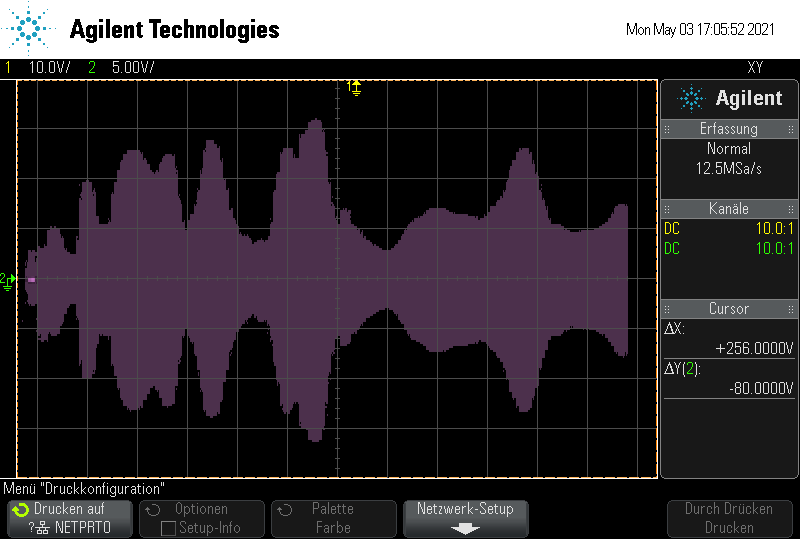
\includegraphics[width=65mm]{Daten/Zyinder/Zylinder_1.png} &   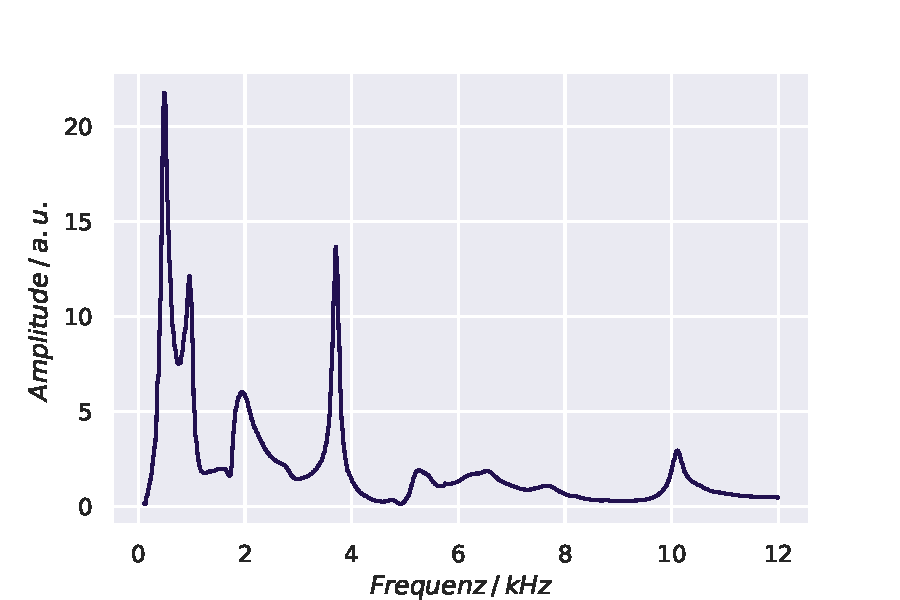
\includegraphics[width=65mm]{Daten/Zyinder/Zylinder_1.pdf} \\
    (a) 1 Zylinder & (b) 1 Zylinder \\[6pt]
     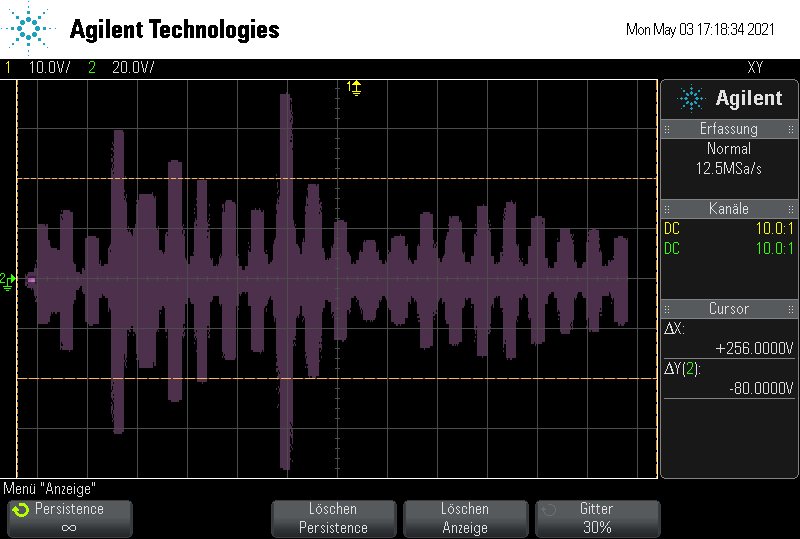
\includegraphics[width=65mm]{Daten/Zyinder/Zylinder_6.png} &   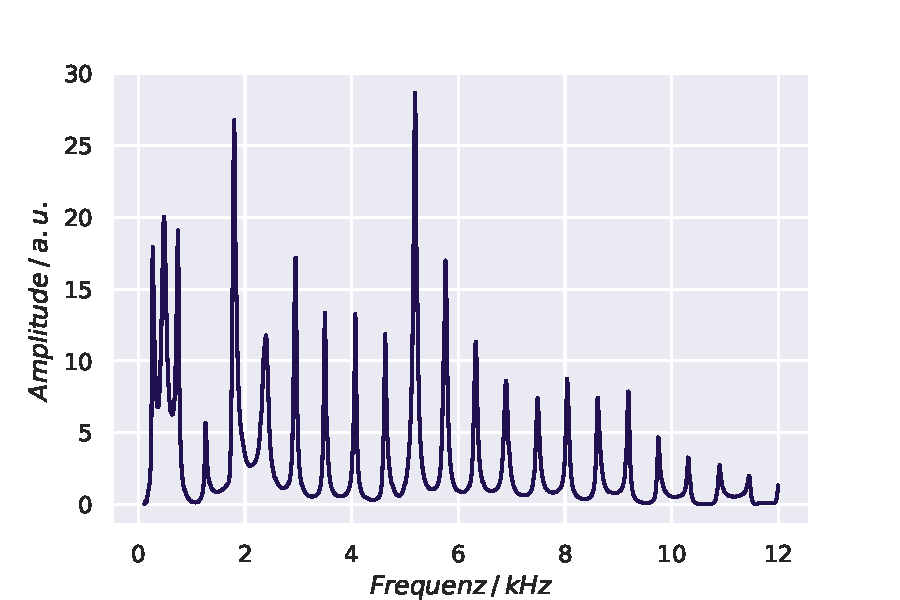
\includegraphics[width=65mm]{Daten/Zyinder/Zylinder_6.pdf} \\
    (c) 6 Zylinder & (d) 6 Zylinder \\[6pt]
    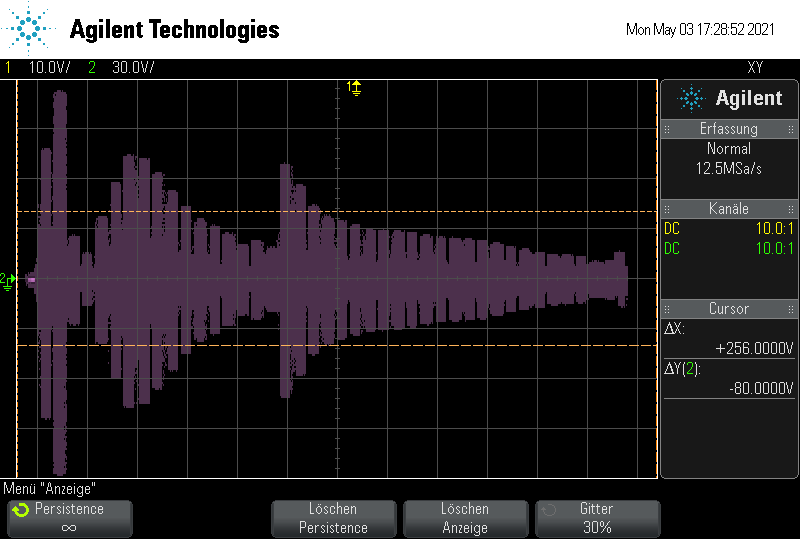
\includegraphics[width=65mm]{Daten/Zyinder/Zylinder_12.png} &   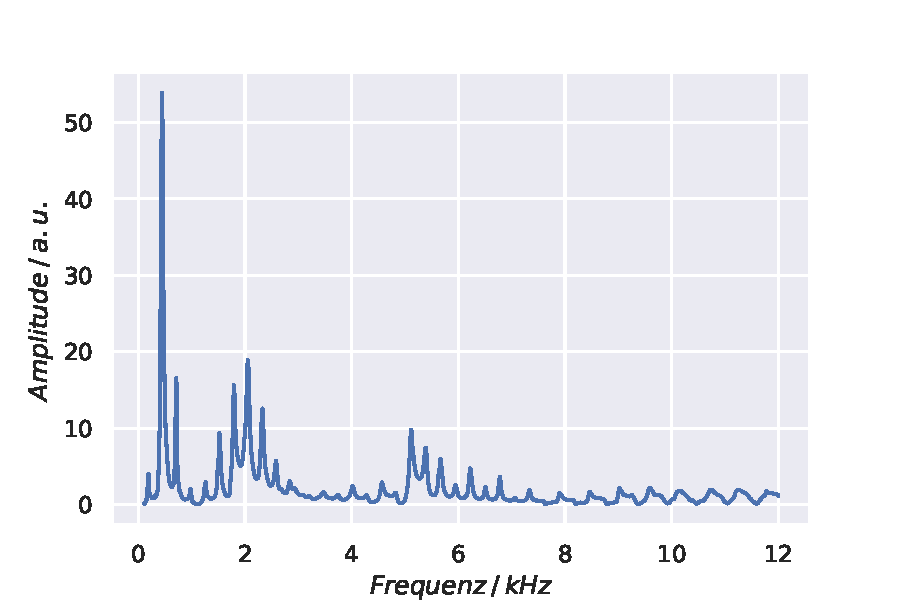
\includegraphics[width=65mm]{Daten/Zyinder/Zylinder_12.pdf} \\
    (c) 12 Zylinder & (d) 12 Zylinder \\[6pt]
    \end{tabular}
    \caption{Gemessene Frequenzspektren der Zylinder-Resonatoren mit unterschiedlicher Länge. Die Messung am Oszillator ist links angegeben und die Messung am Computer rechts. } 
    \label{fig:zyl1-6-12}
\end{figure}

Die Messungen mit dem Oszilloskop zeigen den selben Verlauf wie die Messungen mit dem Computer. Es ist bei allen Messungen das charakteristische Spektrum eines Festkörpers ersichtlich. Die einzelnen Peaks geben die Resonanzen wieder der Zylinderkette. Wie erwartet, nimmt auch die Amplitude mit steigender Frequenz ab. 
Somit bestätigen die Messungen insgesamt die Erwartungen und die Eichung war damit erfolgreich. 
Es ist zu erwähnen, dass die Messung des einzelnen Zylinders ersichtlich nur unsauber gelungen ist. Hier sind die Resonanzen des Zylinders nicht eindeutig erkennbar. Für die weiteren Messungen sind jedoch scharfe Peaks an den Resonanzfrequenzen zu erkennen. \\
Hieran anschließend, wurde das Spektrum eines Zylinders der Länge $75\,\si{\milli\metre}$ aufgenommen. Das Spektrum ist in der Abbildung \ref{fig:fkp75mm} zu sehen.

\begin{figure}[H]
    \centering
    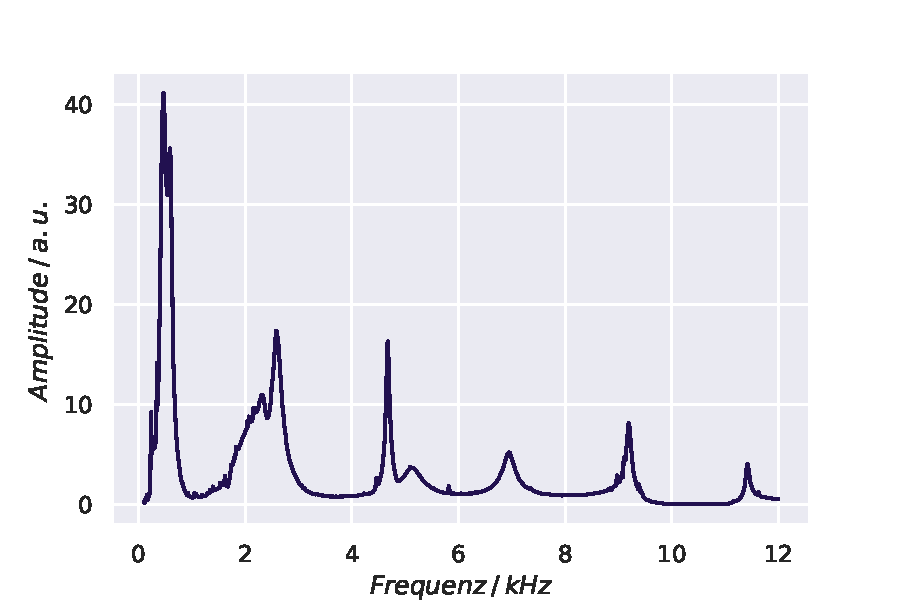
\includegraphics[width=0.8\textwidth]{Daten/Festkörper/FK_75mm.pdf}
    \caption{Das Frequenzspektrum eines $75 \,\si{\milli\metre}$ langen Zylinder-Resonators. }
    \label{fig:fkp75mm}
\end{figure}
An diesem Spektrum sind periodisch auftretende Resonanzen ersichtlich. Die Resonanzen des $75 \,\si{\milli\metre}$ Zylinders müssen an den Frequenzen auftreten, die ca. $\frac{2}{3}$ der Resonanzfrequenzen des $50 \,\si{\milli\metre}$ Zylinders entsprechen. 
Dies folgt aus der größeren Länge des Zylidners. Die stehende Welle des $75 \,\si{\milli\metre}$ Zylinders hat die $1.5$-fache Wellenlänge der stehenden Welle des $50 \,\si{\milli\metre}$ Zylinders. Die Frequenz ist umgekehrt proportional zur Wellenlänge und damit folgt der Faktor $\frac{2}{3}$.

\subsection{Das Wasserstoffatom}
Das Frequenzspektrum des Kugelresonators bei einer Ausrichtung von $\theta = 180°$ wurde mit dem Computer aufgenommen und in der Abbildung \ref{fig:h180} grafisch dargestellt. 
Die beschrifteten Resonanzen werden in der folgenden Analyse für die Berechnung der Druckamplitude verwendet. 
\begin{figure}[H]
    \centering
    \begin{tabular}{c}
    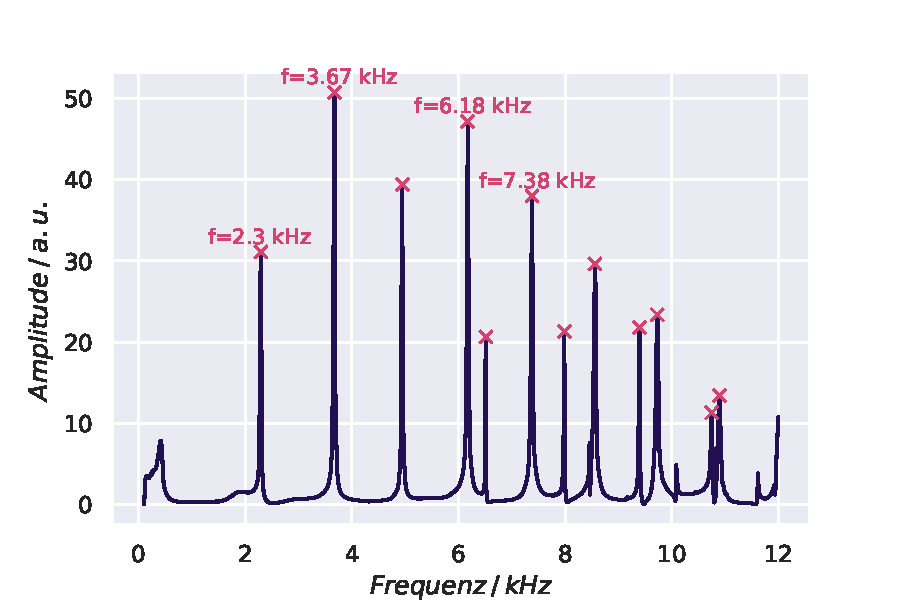
\includegraphics[width=0.9\textwidth]{Daten/Wasserstoff/H_180.pdf} \\
    (a) Messung am Computer \\[6pt]
    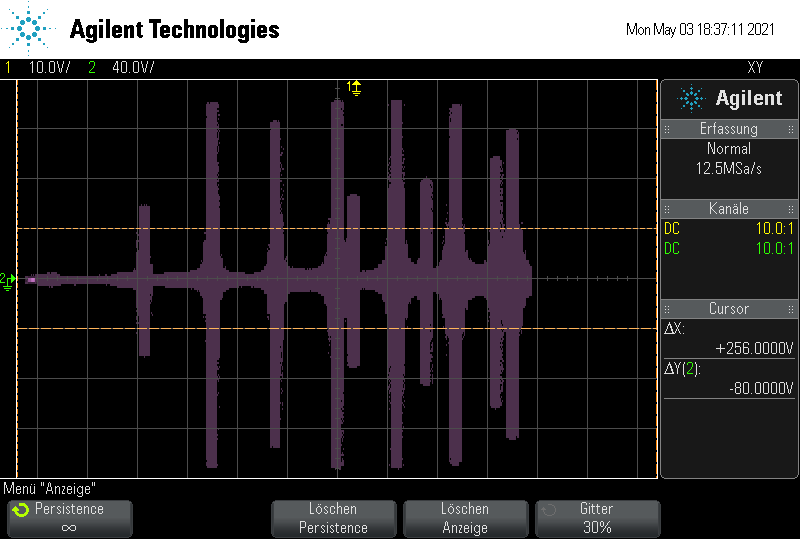
\includegraphics[width=0.9\textwidth]{Daten/Wasserstoff/H_180.png} \\
    (b) Messung am Oszilloskop \\[6pt]
    \end{tabular}
    \caption{Das Frequenzspektrum eines kugelförmigen Hohlraumresonators bei einer Ausrichtung von $\theta = 180\si{°}$ in dem Bereich $0.1 \,\si{\kilo\hertz}$ bis $10 \,\si{\kilo\hertz}$. }
    \label{fig:h180}
\end{figure}

\subsubsection{Druckamplitude}
Für die Berechnung der Druckamplitude mithilfe der gemessenen Werte wird der Ausrichtungswinkel $\theta$ folgendermaßen in den Polarwinkel $\varphi$ umgerechnet:
\begin{align*}
  \varphi = \arccos(\frac{1}{2} \cos(\theta) - \frac{1}{2}).
\end{align*}
Diese Umrechnung folgt aus einer Analyse mit Drehmatrizen \cite{qa-dresden}. Die in Abbildung \ref{fig:h180} beschrifteten Resonanzfrequenzen (also $2.3 \,\si{\hertz}$, $3.67 \,\si{\hertz}$, $6.18 \,\si{\hertz}$ und $7.38 \,\si{\hertz}$) werden nur in Abhängigkeit der Auslenkung in $10°$-Schritten erneut gemessen. 
Die Messung wird in Abhängigkeit des Polarwinkels in Abbildung \ref{fig:hpeaks} aufgetragen. In der selben Abbildung befindet sich der theoretisch erwartete Verlauf bzw. die entsprechenden Legendrepolynome. 
\begin{figure}[H]
  \centering
  \begin{tabular}{cc}
    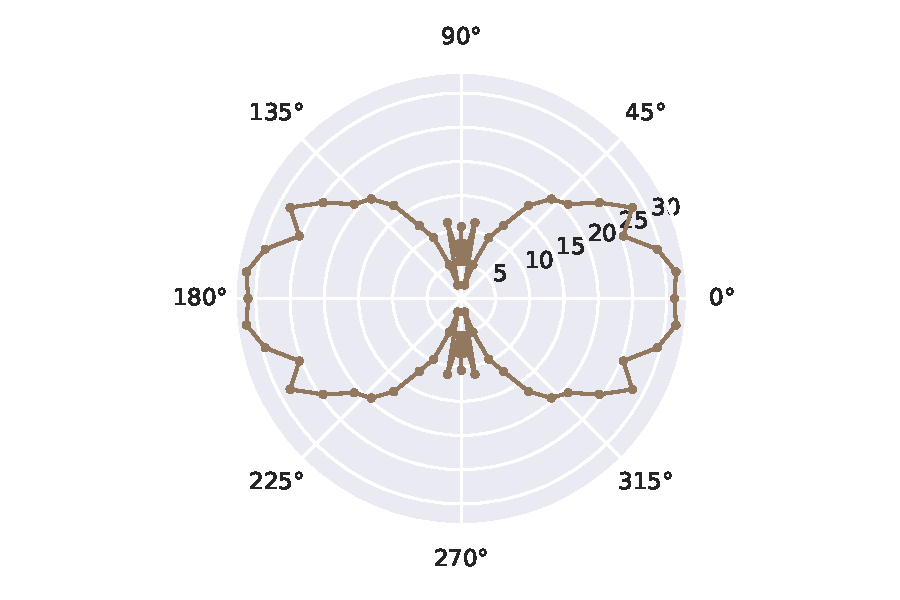
\includegraphics[width=0.5\textwidth]{Daten/Wasserstoff/peak0.pdf} &   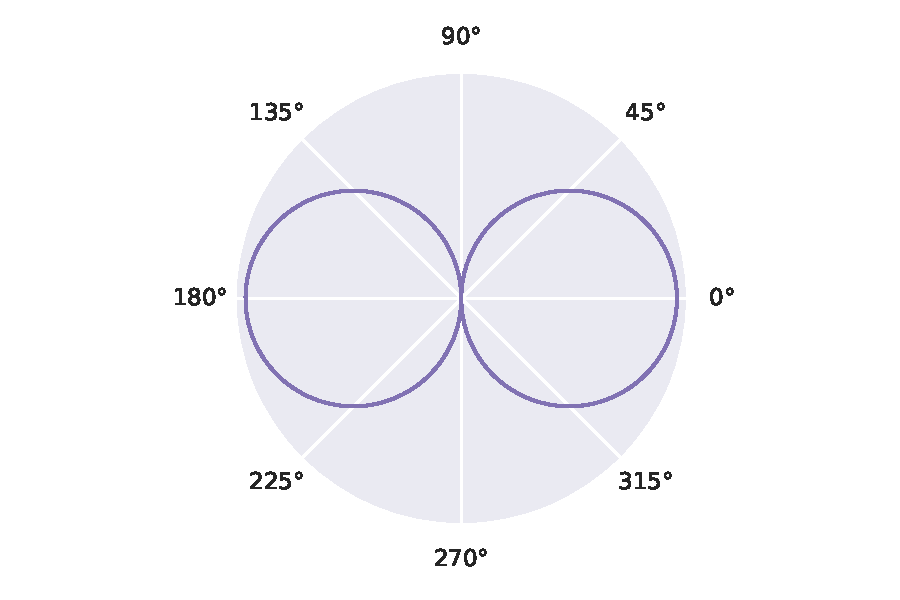
\includegraphics[width=0.5\textwidth]{Daten/Wasserstoff/peakLeg0.pdf} \\
  (a) Resonanz bei $2.3 \,\si{\kilo\hertz} $& (b) $P_1(\cos(\phi))$ \\[6pt]
  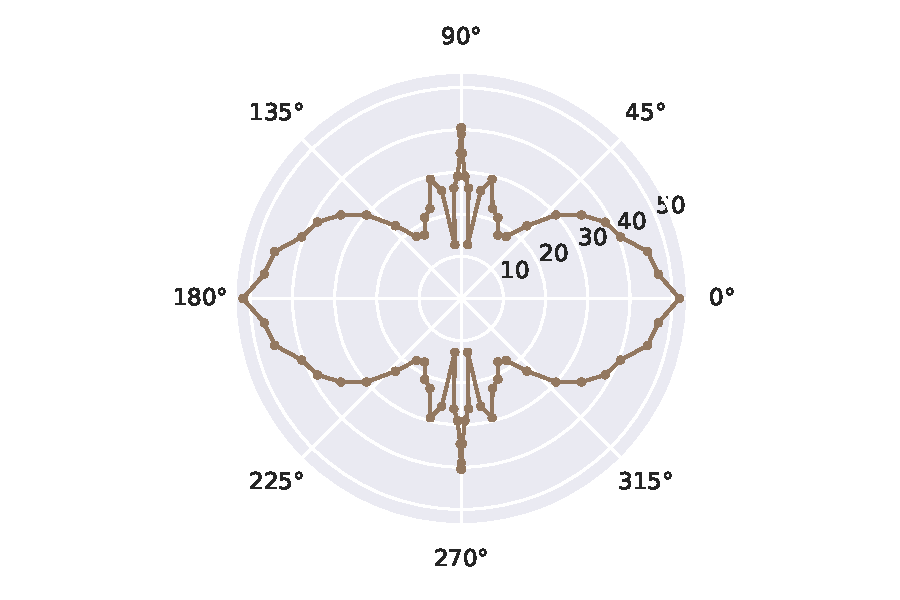
\includegraphics[width=0.5\textwidth]{Daten/Wasserstoff/peak1.pdf} &   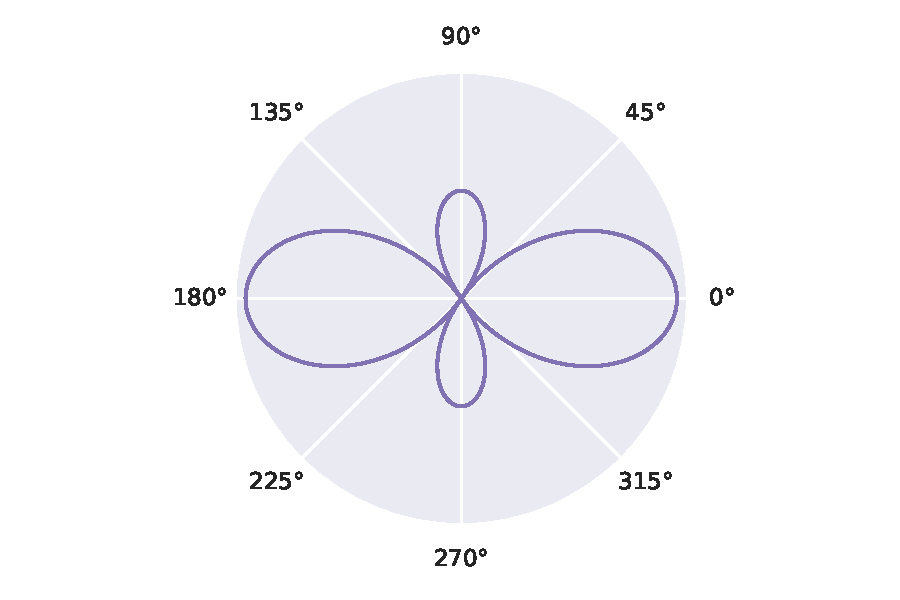
\includegraphics[width=0.5\textwidth]{Daten/Wasserstoff/peakLeg1.pdf} \\
  (c) Resonanz bei $3.67 \,\si{\kilo\hertz}$ & (d) $P_2(\cos(\phi))$ \\[6pt]
  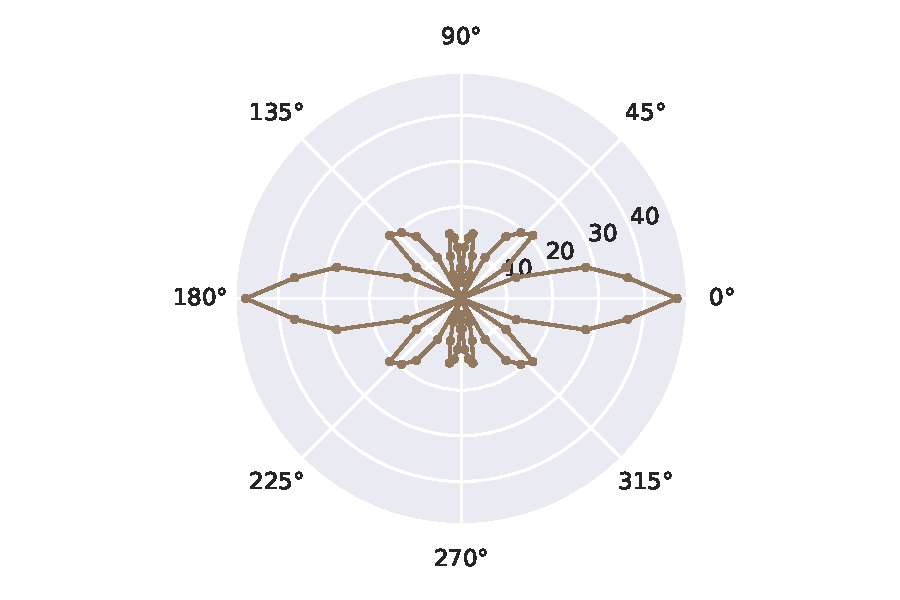
\includegraphics[width=0.5\textwidth]{Daten/Wasserstoff/peak2.pdf} &   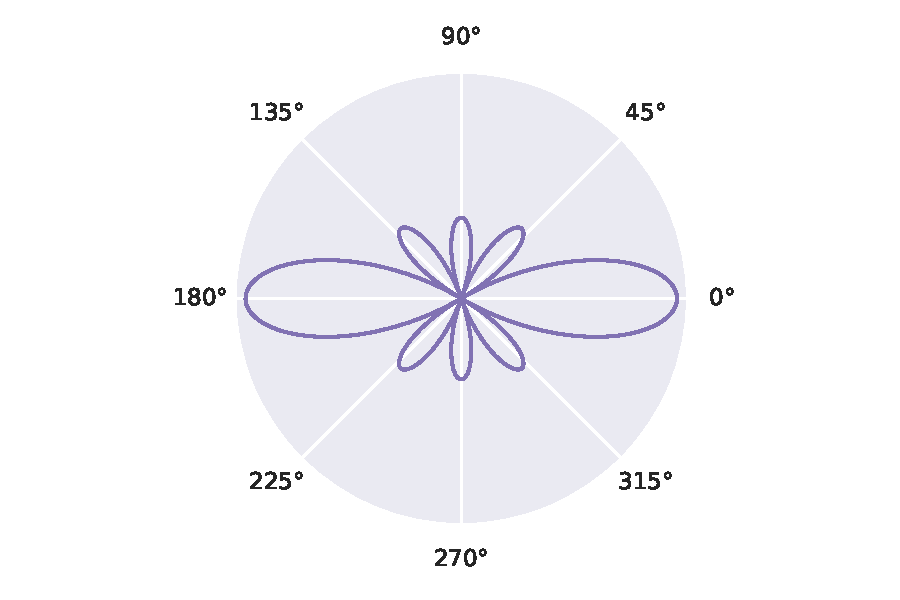
\includegraphics[width=0.5\textwidth]{Daten/Wasserstoff/peakLeg2.pdf} \\
  (c) Resonanz bei $6.18 \,\si{\kilo\hertz}$ & (d) $P_4(\cos(\phi))$ \\[6pt]
  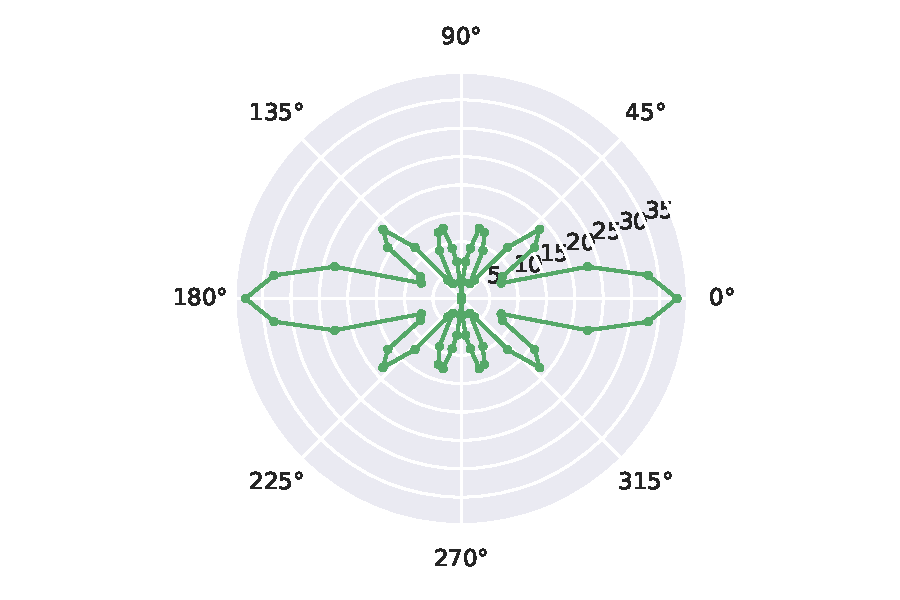
\includegraphics[width=0.5\textwidth]{Daten/Wasserstoff/peak3.pdf} &   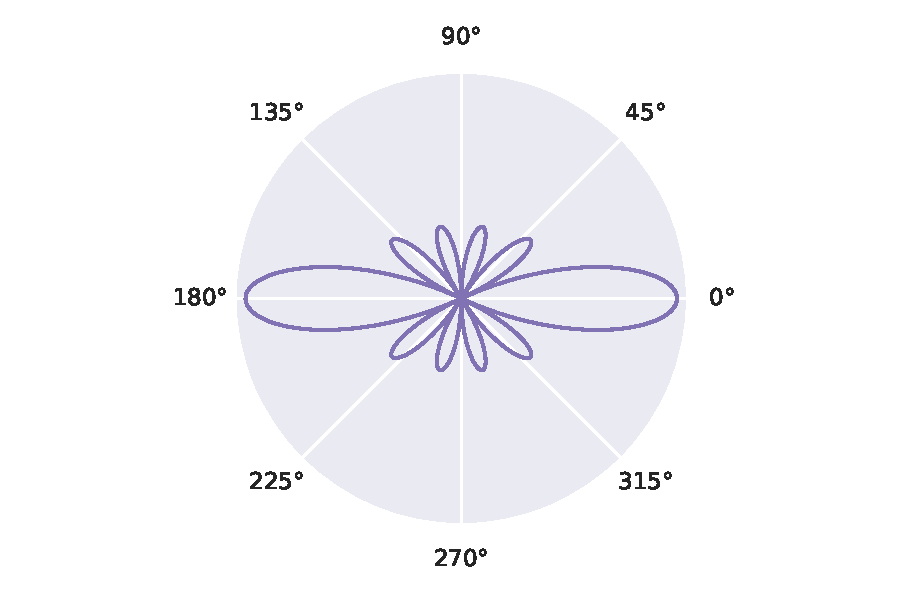
\includegraphics[width=0.5\textwidth]{Daten/Wasserstoff/peakLeg3.pdf} \\
  (c) Resonanz bei $7.38 \,\si{\kilo\hertz}$ & (d) $P_5(\cos(\phi))$ \\[6pt]
  \end{tabular}
  \caption{Amplitudenmessung an den Resonanzfrequenzen in Abhängigkeit vom Azimutwinkel $\phi$ neben der passenden Legendrepolynome. } 
  \label{fig:hpeaks}
\end{figure}
\subsection{Das Wasserstoffmolekül}
\subsection{Festkörper in einer Dimension}